O algoritmo \textit{Simplex} é um método de minimização multidimensional 
sem restrições criado por John A. Nelder e Roger Mead, e publicado em 1965 na revista ``The Computer Journal''.
O método se baseia em utilizar um Simplex para minimizar uma função de $n$ variáveis. 
Mas o que é um simplex? Um Simplex é o menor politopo possível para um espaço de n variáveis. Como exemplo, vemos a figura \ref{fig:simplex}. Para $\mathbb{R}^2$ o menor politopo é um Triângulo, e para $\mathbb{R}^3$ é um Tetraedro.

Este é um método bem generalista que serve para diversos problemas pela sua facilidade, e por não necessitar de Gradientes e Hessianas, como veremos a seguir, é considerado um método de $ordem$ $0$. 

Para facilitar a visualização, representação e entendimento, será explicado o método para $\mathbb{R}^2$ e fica a critério do leitor imaginar para situações com n variáveis.
\begin{figure}[h]
	\begin{center}	
		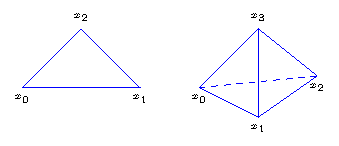
\includegraphics[width=10cm]{simplex/simplex.pdf}
		\caption{Exemplos de Simplex para $\mathbb{R}^2$ e $\mathbb{R}^3$.}
		\label{fig:simplex}
	\end{center}
\end{figure}

\mysubsection{Ordenação}

Com o (novo) Triângulo encontrado, a primeira coisa a se fazer é ordená-lo usando como critério o valor da função $f(x)$ para cada um de seus vértices. Utilizando a mesma nomenclatura de pontos que Nelder e Mead utilizaram em sua publicação, o vértice de menor valor será chamado $x_l$ (de ``low''), o com maior valor será chamado $x_h$ (de ``high'') e o outro ponto iremos chamar arbitrariamente de $x_s$.


\mysubsection{Centróide}

Conhecendo $x_l$, $x_h$ e $x_s$, encontra-se o centróide entre todos os pontos excluindo o $x_h$. O centróide será calculado a partir de

\begin{equation}
c=\dfrac{x_l+x_s}{2}
\end{equation}

\pagebreak
\mysubsection{Reflexão}
Conhecendo $x_l$, $x_h$, $x_s$ e $c$. Calcula-se a reflexão do ponto através da fómula a seguir:

\begin{equation}
x_r=c+\alpha(c-x_h)
\end{equation}

Onde $\alpha$ é chamado índice de reflexão, normalmente igual a $1$.

Podemos ver na figura \ref{fig:reflexao} como realizar a operação graficamente.


\begin{figure}[H]
	\begin{center}	
		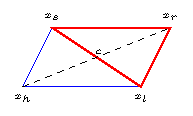
\includegraphics[width=6cm]{simplex/reflexao.pdf}
		\caption{Representação da Reflexão.}
		\label{fig:reflexao}
	\end{center}
\end{figure}

Caso $f(x_l)<f(x_r)<f(x_s)$, $x_h$ é substituído por $x_r$ e a iteração é encerrada. Desse modo verifica-se se algum dos critérios de parada é correspondido e volta-se para a etapa de ordenação.

Caso difira cai-se em algum dos casos das subseções seguintes.

\mysubsection{Expansão}

Se $f(x_r)<f(x_l)$ faz-se a transformação de expansão através da seguinte equação

\begin{equation}
x_e=c+\gamma(x_r-c)
\end{equation}
Onde $\gamma$ é chamado coeficiente de expansão, normalmente igual a $2$.

Podemos ver como realizar a transformação de expansão graficamente na figura \ref{fig:expansao}.



\begin{figure}[H]
	\begin{center}	
		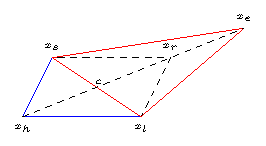
\includegraphics[width=8cm]{simplex/expansao.pdf}
		\caption{Representação da Expansão.}
		\label{fig:expansao}
	\end{center}
\end{figure}

Para terminar a iteração $x_h$ é substituído pelo que possui menor valor de função. Se $f(x_r)<f(x_e)$, aceita-se $x_r$, caso contrário $x_e$ é aceito. Por sempre pegar o menor valor entre os dois, acaba-se eventualmente aumentando o tamanho do triângulo, por isso as vezes o método é chamado de minimização gananciosa, sempre querendo mais e mais .  Depois verifica-se se algum dos critérios de parada é correspondido e volta-se para a etapa de ordenação.

\mysubsection{Contração}
Se $f(x_r)\geq f(x_l)$ faz-se a transformação de Contração através das seguintes equações





\begin{subnumcases}{x_c=}
   c+\beta(x_r-c) & Se $f(x_s)\leq f(x_r)<f(x_h)$ \label{positive}
   \\
   c+\beta(x_h-c) & Se $f(x_r)>f(x_h)$ \label{negative}
\end{subnumcases}

Onde $\beta$ é chamado coeficiente de Contração, normalmente igual a $\frac{1}{2}$.
A contração onde $x_c$ fica entre $x_r$ e $c$ será chamada de \textit{Contração para fora} e a contração onde $x_c$ fica entre $x_h$ e $c$ será chamada de \textit{Contração para dentro}. Cada uma destas transformações podem ser vistas respectivamente da esquerda para direita na figura \ref{fig:contracao}.



\begin{figure}[h]
	\begin{center}	
		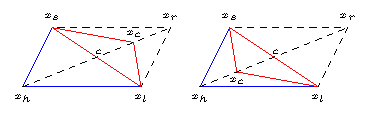
\includegraphics[width=12cm]{simplex/contracao.pdf}
		\caption{Representação das Contrações.}
		\label{fig:contracao}
	\end{center}
\end{figure}

Para encontrar quem ira substituir $x_h$, faz-se algumas comparações pelo ponto mostrado nas equações
\[
\text{Contração para fora}
  \begin{cases} 
    \text{Substituir $x_h$ por $x_c$} & \text{Se } f(x_c)\leq f(x_r) \\
   \text{Realizar encolhimento}       & \text{Se } f(x_c)>f(x_r)
  \end{cases}\]
  \[
  \text{Contração para dentro}
  \begin{cases} 
   \text{Substituir $x_h$ por $x_c$} & \text{Se } f(x_c)<f(x_h) \\
   \text{Realizar encolhimento}       & \text{Se } f(x_c)\geq f(x_h)
  \end{cases}
\]

Caso haja a substituição do ponto termina-se a iteração, verifica-se se algum dos critérios de parada é correspondido e volta-se para a etapa de ordenação.

\pagebreak
\mysubsection{Encolhimento}

O encolhimento é muito raro de acontecer e é usado para quando todas as outras transformações anteriores resultam em pontos cujo valor correspondente na função é pior que os anteriores. O que só acontece em casos específicos. Pode ser visto um extrato da publicação original de 1965, \cite{nelder1965simplex}

\begin{quote}
A failed contraction is much rarer, but can occur when a valley is curved and one point of the simplex is much farther from the valley bottom than the others; contraction may then cause the reflected point to move away from the valley bottom instead of towards it. Further contractions are then useless. The action proposed contracts the simplex towards the lowest point, and will eventually bring all points into the valley.
\end{quote}

Dessa forma a transformação é simplesmente trazer todos os pontos para mais perto do menor, o que pode ser descrito pela equação a seguir

\begin{subequations}
\begin{align}
x_s:=x_s+\delta (x_s-x_l)\\
x_h:=x_h+\delta (x_h-x_l)
\end{align}
\end{subequations} 

Onde $:=$ indica uma substituição do ponto e $\delta$ é chamado coeficiente de encolhimento, normalmente igual a $\frac{1}{2}$.

A transformação pode ser vista na figura \ref{fig:encolher}, onde em vermelho é o novo triângulo formado.

\begin{figure}[h]
	\begin{center}	
		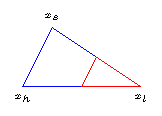
\includegraphics[width=6cm]{simplex/encolher.pdf}
		\caption{Representação do Encolhimento.}
		\label{fig:encolher}
	\end{center}
\end{figure}

Depois de substituídos os pontos termina-se a iteração, verifica-se se algum dos critérios de parada é correspondido e volta-se para a etapa de ordenação.

\pagebreak
\mysubsection{Critérios de Parada}

O primeiro critério de parada mais simples é o número de iterações realizadas, o que não precisa de explicações.
O segundo critério, foi uma maneira de distinguir o quanto os pontos do triângulo estão próximos um do outro, assim
encontra-se o circuncentro do triângulo e o raio do da circunferência circunscrita denota a distância entre os vértices, quando ele for menor que um certo valor termina-se a minimização.

\begin{figure}[H]
	\begin{center}	
		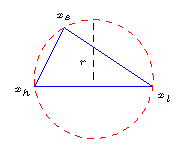
\includegraphics[width=8cm]{simplex/parada.pdf}
		\caption{Circunferência circunscrita ao simplex.}
		\label{fig:parada}
	\end{center}
\end{figure}


Já o terceiro critério foi o mesmo utilizado na publicação original. Procura-se o desvio padrão de todos os valores de $f(x)$ encontrados de modo a ter uma pequena ideia de como é a superfície. Quando o desvio chega a zero significa que a superfície se comporta como um plano que não possui mínimo. então como eles dizem em \cite{nelder1965simplex}

\begin{quote}
The success of the criterion depends on the simplex not becoming too small in relation to the curvature of the surface until the final minimum is reached.
\end{quote} 

Escolhe-se um desvio tão pequeno quanto se queira para ser referência e uma vez que o desvio da superfície decresça e se torne menor que ele, termina-se a minimização


\newpage

